% DOCUMENT TITLE
% main.tex
% Template: Jake Davis, Tyler Holliday, Ryan Barna
% Author:   Sarah Pawlowsk 
% Created:  January 9 2024

% Initialize
%------------------------------
\documentclass[12pt]{article}
\usepackage[scaled]{helvet}
\usepackage[utf8]{inputenc}
\usepackage[T1]{fontenc}
\usepackage{geometry}
\usepackage[english]{babel}
\usepackage{graphicx}
\usepackage{ragged2e} % add [document] to set entire document to the text alignment
\usepackage{float}
\usepackage{textpos}
\usepackage{setspace}
\usepackage{tocloft}
\usepackage[skip=12pt]{parskip}
\usepackage{wrapfig}
\usepackage{xhfill}
\usepackage{enumitem}
\usepackage{caption}
\usepackage{hyperref}
\usepackage{booktabs}
\usepackage{array}
\usepackage{longtable}
\usepackage[font={small,it}]{caption}
\usepackage[autostyle, english = american]{csquotes}
\usepackage{xcolor,colortbl}
\usepackage{tcolorbox}
\usepackage[nopostdot,nogroupskip=true,acronyms,nonumberlist=true]{glossaries}
\usepackage{pageslts}
\usepackage{fancyhdr}
\usepackage{color}
\usepackage[backend=biber,sorting=none]{biblatex}
\usepackage{arrayjobx}
\usepackage{pgffor}
\usepackage{draftwatermark} %un-comment for DRAFT watermark, see below for other stuff that needs to be un-commented as well

\addbibresource{sections/references.bib}

\renewcommand\familydefault{\sfdefault}

\makenoidxglossaries
\setglossarystyle{long}

\renewcommand{\glsnamefont}[1]{\textbf{#1}}

\captionsetup{justification=centering,singlelinecheck=false,format=hang} % Centers captions

\geometry{letterpaper, margin=1in} % Sets up the page size and margins

\graphicspath{ {images/} } % Defines the folder to look for images in

\pagenumbering{arabic} % Defines page numbering scheme

\pagestyle{fancyplain}
\renewcommand\plainheadrulewidth{.4pt}
\renewcommand\plainfootrulewidth{.4pt}

\renewcommand\arraystretch{1.5}

% TABLE COLUMNS, use C{1in} to define a centered column 1 inch wide.
%------------------------------
\newcommand{\PreserveBackslash}[1]{\let\temp=\\#1\let\\=\temp}
\newcolumntype{C}[1]{>{\PreserveBackslash\centering}p{#1}}
\newcolumntype{R}[1]{>{\PreserveBackslash\raggedleft}p{#1}}
\newcolumntype{L}[1]{>{\PreserveBackslash\raggedright}p{#1}}
%------------------------------


% Variables to change depending on the project
%------------------------------
\newcommand{\programName}{ASIO}
\newcommand{\docType}{Engineering Model Test Document}
\newcommand{\docTitle}{Background Noise Tests}
\newcommand{\docAbr}{ASIO TEST}
\newcommand{\docNum}{ASIO-TEST-0022}
\newcommand{\docDate}{08/26/2025}
\newcommand{\dateEdit}{08/26/2025}
\newcommand{\revNum}{0.0}

% signers (can have up to six on a single page)
\newcommand{\signersCount}{6}

\newcommand{\firstName}{Name One}
\newcommand{\firstNameTitle}{Title/Role}
\newcommand{\firstNameOrg}{Institution}

\newcommand{\secondName}{Name Two}
\newcommand{\secondNameTitle}{Title/Role}
\newcommand{\secondNameOrg}{Institution}

\newcommand{\thirdName}{Name Three}
\newcommand{\thirdNameTitle}{Title/Role}
\newcommand{\thirdNameOrg}{Institution}

\newcommand{\fourthName}{Name Four}
\newcommand{\fourthNameTitle}{Title/Role}
\newcommand{\fourthNameOrg}{Institution}

%------------------------------

% ACRONYMS
%------------------------------
\newacronym{SSEL}{SSEL}{Space Science and Engineering Laboratory}
\newacronym{MSU}{MSU}{Montana State University}
\newacronym{ACY}{ACY}{Acronym}
\newacronym{ND}{ND}{Neutral Density}
\newacronym{SXR}{SXR}{Soft X-ray}
\newacronym{HXR}{HXR}{Hard X-ray}
\newacronym{EUV}{EUV}{Extreme Ultra Violet}
\newacronym{FFT}{FFT}{Fast Fourier Transform}
\newacronym{LM}{LM}{Lockheed Martin}
\newacronym{SNR}{SNR}{Signal to Noise Ratio}
\newacronym{EM}{EM}{Engineering Model}
\newacronym{GSE}{GSE}{Ground Support Equipment}
\newacronym{CPT}{CPT}{Comprehensive Performance Test}
\newacronym{ICD}{ICD}{Interface Control Document}
%------------------------------

\glsunsetall

% WATERMARK, un-comment to add DRAFT watermark to the first page
%-------------------------------
\SetWatermarkText{DRAFT}
\SetWatermarkScale{0.5}
\SetWatermarkAngle{0}
\DraftwatermarkOptions{vpos=0.35\paperheight}
%------------------------------

% BEGIN DOCUMENT
%------------------------------
\begin{document}
    
    \setlength{\parindent}{0pt}
\begin{titlepage}
    % Page setup
    %------------------------------
    % program logo
    \begin{minipage}{.22\textwidth}
        \begin{flushleft}
            
\includegraphics[height=1.2in]{mission_logo.png}
        \end{flushleft}
    \end{minipage}
    % program name/info
    \begin{minipage}{.54\textwidth}
        \centering
        \large\textbf{\programName \\ \vspace*{6pt} \docType}
        %\hfill
    \end{minipage}
    % nasa logo
    \begin{minipage}{.22\textwidth}
        \begin{flushright}
            
\includegraphics[height=1in]{nasa-logo.png}
        \end{flushright}
    \end{minipage}
    % doc info
    \vspace{0.35in}

    \textbf{Date:~} \dateEdit \hfill \textbf{Document Number:~} \docNum \vspace{12pt}

    \hrule height 1.5pt
    
    \vspace{1.5in}

    \begin{center}
        \LARGE{\textbf{\docTitle}}\\ \vspace{.25in}
    \begin{table}[h!]
	\centering
    \begin{tabular}{m{1in} m{1in}}
	Test Date: & \\
	\hline
    \end{tabular}
    \end{table}
    \end{center}
    
    \vspace{0.5in}

    % SSEL logo
    \begin{minipage}{\textwidth}
        \centering
        
\includegraphics[width=2.5in]{sselbanner_square.png}
    \end{minipage}
    
    %\vspace{0.5in}
    
    %Reason for Test: \rule{3in}{1pt} \hfill Date: \rule{1in}{1pt}
    
    \vfill
    %------------------------------

	\hrule height 1.5pt
	
	\begin{minipage}{0.55\textwidth}
		\textbf{Montana State University} \\
		\textbf{Space Science and Engineering Laboratory}
	\end{minipage}
    \hfill
	\begin{minipage}{0.45\textwidth}
		\hfill 
\includegraphics[height=0.5in]{MSU.jpg}
	\end{minipage}
\end{titlepage}
    \newpage

    %\DraftwatermarkOptions{stamp=false} - Un-comment to only have watermark on the first page (recommended because the watermark does not go over images)

    \newgeometry{top=1.25in,left=1in,right=1in,bottom=1in,headheight=0.8in,headsep=24pt}

    \pagestyle{fancy}
    \fancyhf{}
    \fancyhead[L]{\textcolor{gray}{\docAbr} \vspace{6pt}}
    \fancyhead[C]{\textcolor{gray}{\docNum} \vspace{6pt}}
    \fancyhead[R]{\textcolor{gray}{\dateEdit} \vspace{6pt}}
    \fancyfoot[R]{Page: \hspace{6pt} \thepage \hspace{6pt} of \hspace{6pt} \lastpageref{LastPage}}
    \fancyfoot[L]{\textcolor{gray}{Revision~\revNum}}
    \renewcommand{\headrulewidth}{0.4pt}
    \renewcommand{\footrulewidth}{0.4pt}

	\newpage

    % revision log
    %\section*{Revision Log}
    %% DOCUMENT NAME
% revision_log.tex
% Template: Jake Davis, Tyler Holliday, Ryan Barna
% Author:
% Created:


%% begin log
\begin{table}[H]
    \centering
    \begin{tabular}{C{0.35in}|p{2.85in}|C{1in}|C{1.4in}}
    	\textbf{Rev.} & \textbf{Purpose/Change} & \textbf{Date} & \textbf{Approval} \\ \hline
        0.0 & Document created & 01/01/2024 & Approver Name \\ 
        0.1 & Document changed for XYZ & 01/01/2024 & Approver Name \\ 
    \end{tabular}
    \label{tab:rev}
\end{table}

    %\newpage

    %% Tables %%
    \setstretch{1.15}
    \renewcommand{\contentsname}{TABLE OF CONTENTS}
    \renewcommand{\listfigurename}{LIST OF FIGURES}
    \renewcommand{\listtablename}{LIST OF TABLES}

    % table of contents
    \setcounter{table}{0}
    \tableofcontents\thispagestyle{fancy}
    \newpage

    % list of figures
    \listoffigures\thispagestyle{fancy}
    \vspace*{.35in}
    
    % list of tables
    \listoftables\thispagestyle{fancy}

    % list of acronyms
    \setlength\LTleft{10pt}
    \setlength\LTright{0pt}
    \setlength\glsdescwidth{0.8\hsize}
    \glsaddall
    \printnoidxglossary[type=acronym,title=LIST OF ACRONYMS]\thispagestyle{fancy}
    \newpage

    \setcounter{table}{0}
    \setcounter{figure}{0}

    \captionsetup{belowskip=0pt}
    \captionsetup{aboveskip=10pt}

    % setup row counter for step-based table
    \newcounter{step_num}
    \newcommand\rownumber{\thesubsection.\stepcounter{step_num}\arabic{step_num}} % if need to include more or less subheadings in the number just add or remove additional 'sub's to \thesubsection (i.e. \thesubsubsection)
    
    
    % INPUT SECTIONS HERE
    % -------------------------------------------------------------------------------------------------
    
    % Testing Plan Overview
% 01_section.tex
% Author: Sarah Pawlowski 
% Date: 1/12/25

%% begin text
\section{Introduction}
The purpose of this document is to outline the testing procedure for the background noise test
of the ASIO instrument. These tests are meant to establish a baseline background noise level
that will be used as a comparison for future tests run on the instrument, refer to the ASIO
MSU Testing Overview (BUBO-TEST-0012) for descriptions of these tests. Additionally, these
tests are a first indicator if the housing of ASIO is light-tight before completing more rigorous
and specific light-tightness tests. An ESD safe smock, grounding bracelet and grounding strap
should be worn while handling ASIO.

\subsection{Required Testing Equipment}
\begin{table}[h!]
	\centering \caption{Testing Equipment}
	\begin{tabular}{|c|}
		\hline
		\textbf{Required Equipment} \\
		\hline
	ASIO Instrument \\
        External Computer \\
        Ground Support Software \\
        Cables \\
        Keysight E36313A Bench Power Supply \\
        RS422 to USB converter \\
        11 -  Thorlabs SM1CP2 end caps \\
        Dark Box \\
        ESD safety Equipment \\
        \hline
	\end{tabular}
\end{table}

\subsection{Test Engineer(s)}
\begin{table}[H]
	\centering
	\begin{tabular}{p{2in} p{2in} p{2in}}
		& & \\
		& & \\ \hline
		Test engineer & Signature & Date \\
		& & \\
		& & \\ \hline
            Test engineer & Signature & Date \\
            & & \\
		& & \\ \hline
            Test engineer & Signature & Date \\
	\end{tabular}
\end{table}

\subsection{Instrument Description}
The diagrams below show the the connectors and the front face of the ASIO instrument. See the ICD (BUBO-SYSE-0001) for the full pinout details of each connector and more details on how to interface with each connector correctly.

\begin{figure}[H] 
    \centering
    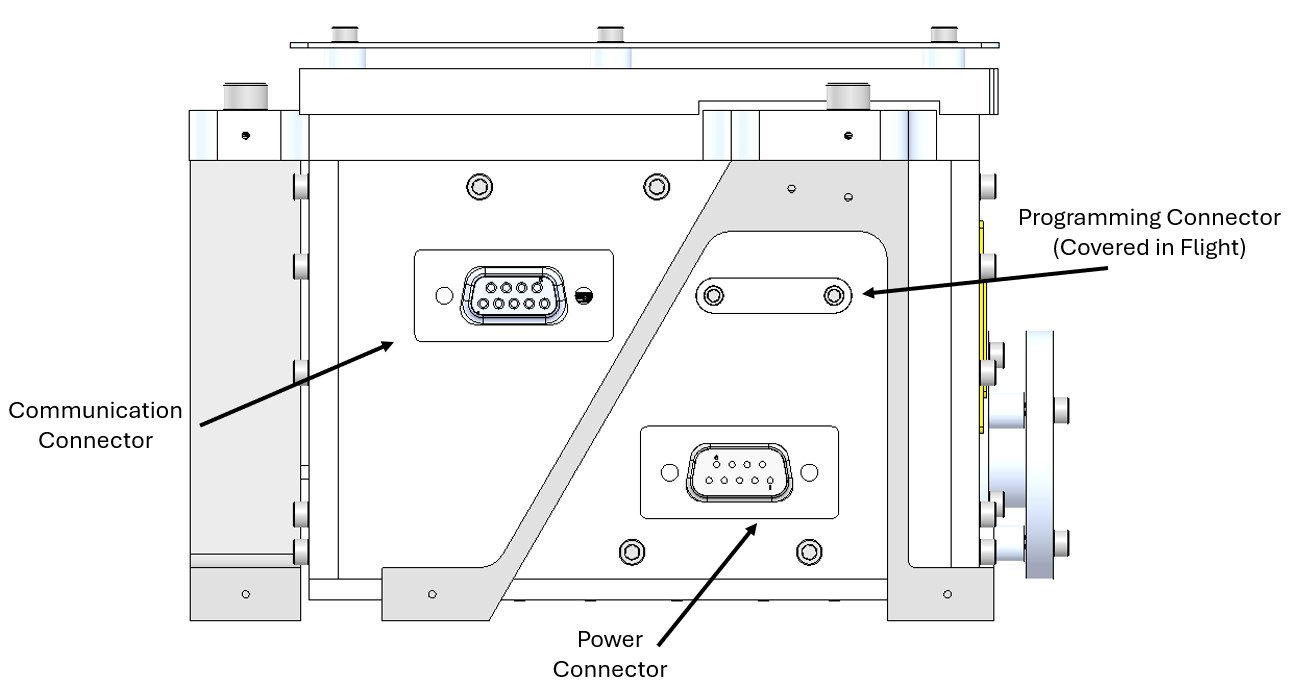
\includegraphics[width=6in]{images/BUBO - connector interface.jpg}
    \caption[ASIO Connector Interface], {ASIO Connector Interface when ASIO is mounted on the optical bench for testing the vent is facing down towards the bench. This makes the communication connector the port above the power connector.}
    \label{fig:ASIO Connector Interface}
\end{figure}

The detectors are numbered as shown in figure \ref{fig:LabeledDetectors} below. These background noise tests are conducted on the ASIO instrument as a whole, rather than individual photodiodes or channels. This figure is for reference only and will not be used to label datasets.

\begin{figure}[H] 
    \centering
    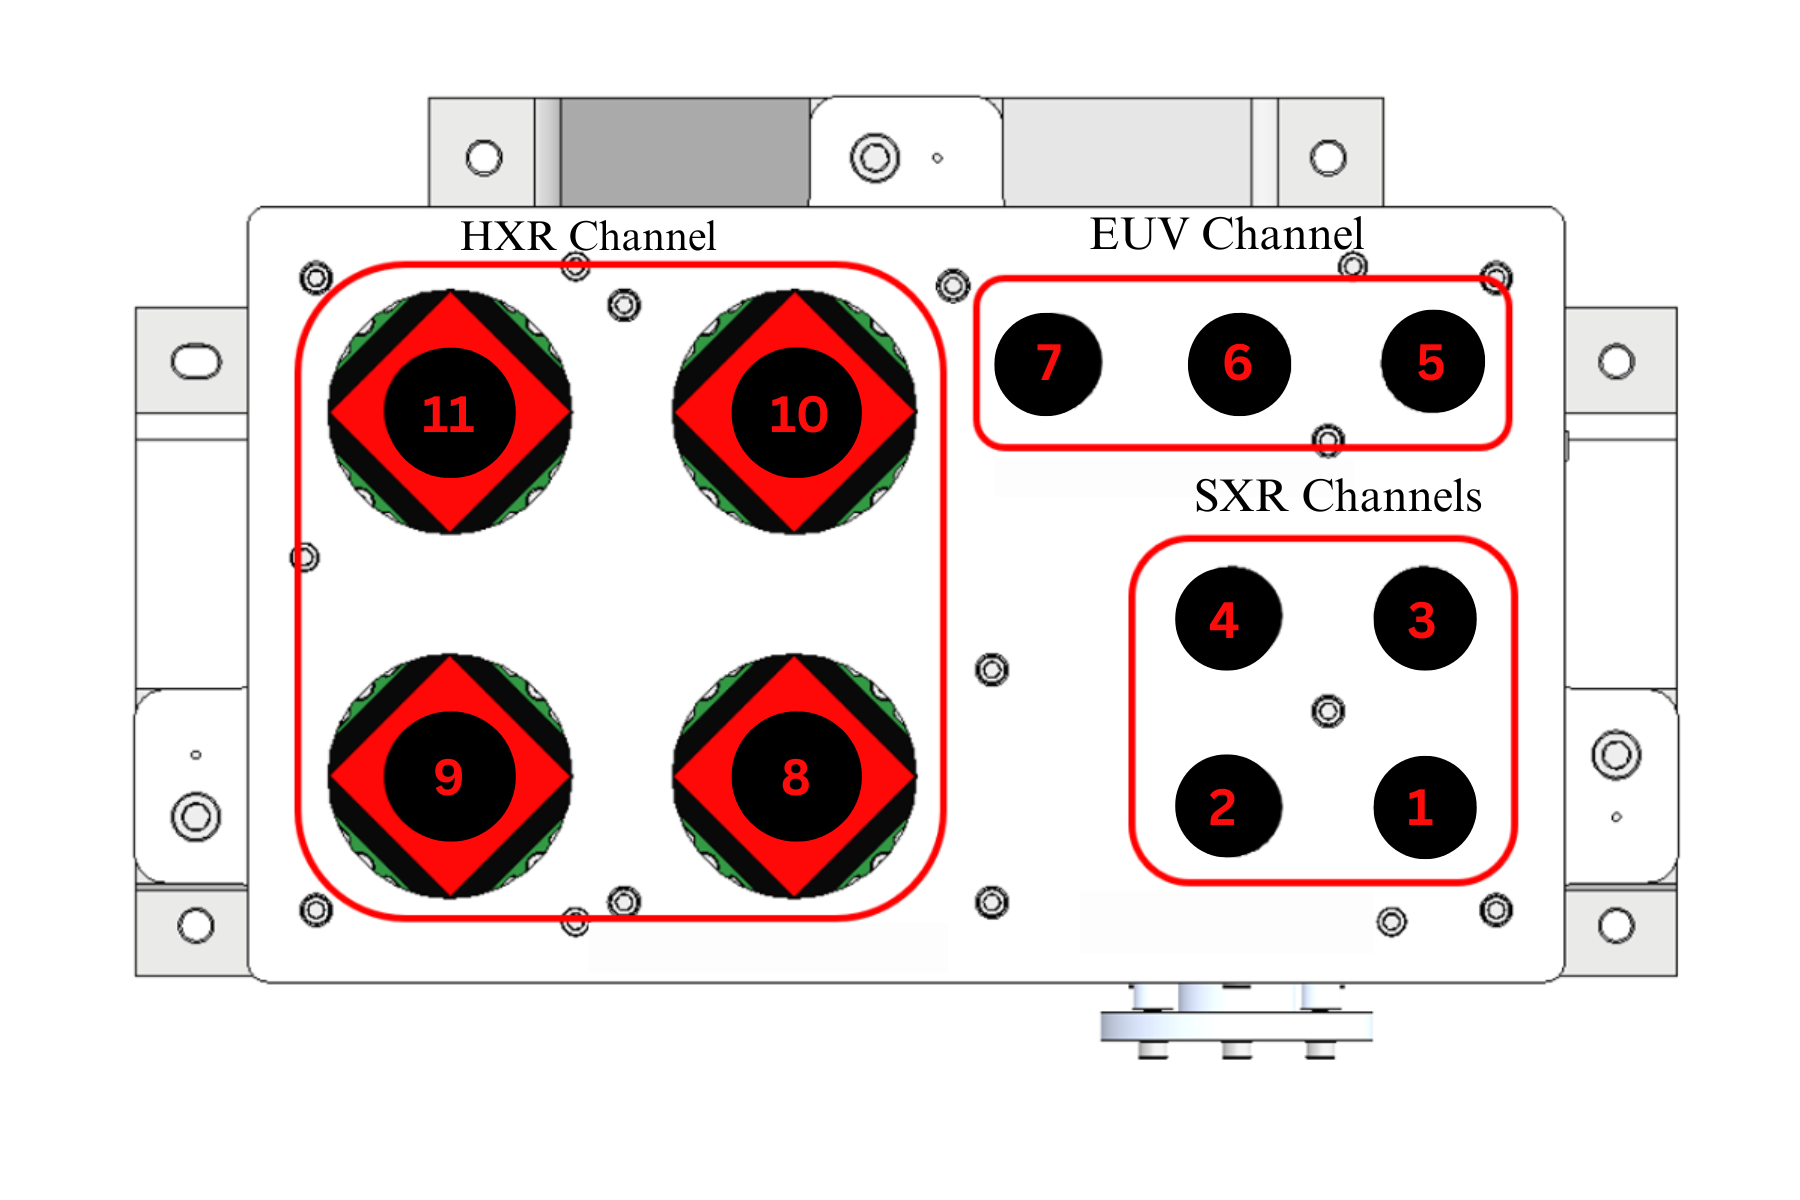
\includegraphics[width=6.5 in]{images/Photodiode_Diagram.png}
    \caption[ASIO Detector Labels]{ASIO Detector Labels, oriented in the same direction instrument is connected to optical bench.}
    \label{fig:LabeledDetectors}
\end{figure}


    % Testing Plan Overview
% 02_section.tex
% Author: Sarah Pawlowski
% Date: 1/14/25

%% begin text
\section{Limited Performance Test (LPT)}

This test includes portions of sections 2 and 3.1 of the Comprehensive Performance Test
(CPT), document ASIO-SYSE-0016. These tests are done as a quick evaluation that the in-
strument is functioning as expected and to establish a baseline before collecting data associated with a test on the EM. All photodiodes should be capped for this test, they can be performed with lights on or off in lab 244 or the SSEL.

\subsection{Test Setup}

\newcolumntype{C}[1]{>{\centering\arraybackslash}p{#1}}

\begin{center}
\begin{longtable}{|C{0.3in}|m{4.25in}|C{0.75in}|} 
\caption{Test Setup Guide - Step by Step} \\
\hline
\# & \textbf{Description} & \textbf{Initials} \\
\hline
\endfirsthead

\hline
\# & \textbf{Description} & \textbf{Initials} \\
\hline
\endhead

\hline
\multicolumn{3}{r}{\emph{Continued on next page}} \\
\endfoot

\hline
\endlastfoot

2.1 & Set the bench power supply to output +28 V. Set the current limit to 200 mA (0.2 A). Make sure the output is off. & \\ 
\hline
2.2 & Make sure that all test engineers are wearing ESD smocks and grounding wrist straps. Follow ESD protection protocols throughout the testing process. & \\ 
\hline
2.3 & Plug the ASIO communication cable into the communication D-Sub connector. Reference figure \ref{fig:ASIO Connector Interface}.& \\ 
\hline
2.4 & Plug the RS422 into the ASIO communication cable and the testing computer. & \\ 
\hline
2.5 & Attach the bench supply cables to the correct pins in the ASIO power D-Sub connector. Reference figure \ref{fig:ASIO Connector Interface}.& \\ 
\hline
2.6 & Make sure that the bench supply power cables are separated and will not short at any point during this test. & \\ 
\hline
\end{longtable}
\end{center}

\subsection{Electrical Tests}

\newcolumntype{C}[1]{>{\centering\arraybackslash}p{#1}}

\begin{center}
\begin{longtable}{|C{0.3in}|m{3.25in}|C{1in}|C{0.75in}|}
\caption{Electrical Test Guide - Test Setup} \\
\hline
\# & \textbf{Electric Test Setup} & \textbf{Expected/ Measured} & \textbf{Initials} \\
\hline
\endfirsthead

\hline
\# & \textbf{Electric Test Setup} & \textbf{Expected/ Measured} & \textbf{Initials} \\
\hline
\endhead

\hline
\multicolumn{4}{r}{\emph{Continued on next page}} \\
\endfoot

\hline
\endlastfoot

2.21 & Start the testing software on the computer. & NA &  \\
\hline
2.22 & Enable the +28V output on the bench power supply. \textbf{Record the current} output of the bench supply about ten seconds after turn-on. & 
\begin{tabular}{l}
62mA$\pm$10mA \\
value:
\end{tabular} & \\
\hline
2.23 & Record the temperatures from ASIO's internal censors, found in health data of the ASIO packet. This should be displayed by the GSE. & & \\
\hline
2.24 & Record the digital system \textbf{current} measured by the ASIO instrument, found in the health data of the ASIO packet. This should be displayed by the GSE. &
\begin{tabular}{l}
32mA$\pm$5mA \\
value:
\end{tabular} & \\
\hline
2.25 & Record the bus \textbf{voltage} measured by the ASIO instrument. This is found in the health data of the ASIO packet and should be displayed by the GSE. & 
\begin{tabular}{l}
3.3V$\pm$0.05V \\
value:
\end{tabular} & \\
\hline
2.26 & Verify that the ASIO instrument is sending packets to the testing computer about once every 0.5 seconds, use the packet counter found in the health data of the ASIO packet and should be displayed by the GSE. & YES & \\
\hline
2.27 & Collect and analyze a 5 minute dataset with no signal input to establish a baseline. Record the mean and std dev for each channel in the table below. & NA & \\
\hline

\end{longtable}
\end{center}

\begin {center}
\begin{longtable}{|C{0.7in}|C{1.5in}|C{1.5in}|C{1.8in}|}
\caption{Baseline Data Table} \\
\hline
\textbf{Channel} & \textbf{Mean Expected (V)} & \textbf {Mean Measured (V)} & \textbf{Std Dev Measured (V)} \\
\hline
\endfirsthead

\hline
\textbf{Channel} & \textbf{Mean Expected (V)} & \textbf {Mean Measured (V)} & \textbf{Std Dev Measured (V)} \\
\hline
\endhead

\hline
\multicolumn{4}{r}{\emph{Continued on next page}} \\
\endfoot

\hline
\endlastfoot

\textbf{SXR1} & $6.08339e^-3$ & & \\
\hline
\textbf{SXR2} & $6.02614e^-3$& & \\
\hline
\textbf{SXR3} & $6.04632e^-3$& & \\
\hline
\textbf{SXR4} & $5.96000e^-3$ & & \\
\hline
\textbf{HXR} & $6.13372e^-3$ & & \\
\hline
\textbf{EUV} & $6.00174e^-3$& & \\
\hline

\end{longtable}
\end{center}

\textit{$^*$Note: These expectation values were calculated using Background\_Noise\_Expectations.py which is located on Gitlab in the science branch under testing-results/analysis/04\_EM\_Testing. These should be updated with each new configuration of ASIO and will require ASIO Background Noise Test to be repeated.}

\newpage


    
    \section{Background Noise Tests}
\subsection{Background Noise Tests - 10 Minute Datasets}
This portion of the test should be completed in its entirety immediately after section 2. All photodiodes must be capped for this test, three of the ten minute tests should be run with the lab lights, three should be run with the lab lights off, and three should be run with ASIO in a dark box and the lab lights off.


\newcolumntype{C}[1]{>{\centering\arraybackslash}p{#1}}

\begin{center}
\begin{longtable}{|C{0.3in}|m{3.25in}|C{1.75in}|}
\caption{Background Noise Test 10 Minute Datasets Guide - Step by Step} \\
\hline
\# & \textbf{Description} & \textbf{Notes}  \\
\hline
\endfirsthead

\hline
\# & \textbf{Description} & \textbf{Notes} \\
\hline
\endhead

\hline
\multicolumn{3}{r}{\emph{Continued on next page}} \\
\endfoot

\hline
\endlastfoot

3.1 & Start with room lights on, start the testing software on the computer. & \\
\hline
3.2 & Collect a 10 minute dataset, verify that mean and standard deviation meets expectations using the GSE software. Record the mean and standard deviation in the table below. & \\
\hline
3.3 & Repeat this process two additional times for a total of three datasets. & \\
\hline
3.4 & Clearly name datasets, include a number to keep data in chronological order, date (YYYYMMDD), test type, and trial.
Example: 01\_20250818\_background\_lights\_1.csv
 & \\
\hline
3.5 & Repeat step 3.2, 3 additional times with the lab room lights off. Record the mean and standard deviation for each in the table below. & \\
\hline
3.6 & Switch the short comms cable with the longer comms cable for the dark box testing, this way the RS-422 to USB converter can be outside the dark box. & \\
\hline
3.7 &  Repeat step 3.2, 3 additional times with the lab room lights off and with ASIO in a dark box. Record the mean and standard deviation for each trial in the table below. & \\
\hline
3.8 & Store all test datasets in a clearly labeled file that includes test name and date. Upload a copy to GitLab under the science testing results section (MUSE/Science/testing-results) under the Labtop branch. Refer to the README in the testing-results repo for organization  & \\
\hline

\end{longtable}
\end{center}



\begin {center}
\begin{longtable}{|C{1in}|C{2in}|C{2in}|}
\caption{Background Noise 10 Minute Data Collection Table} \\
\hline
\textbf{Test} & \textbf {Mean (V)} & \textbf{Std Dev (fA)} \\
\hline
\endfirsthead

\hline
\textbf{Test} & \textbf {Mean (V)} & \textbf{Std Dev (fA)} \\
\hline
\endhead

\hline
\multicolumn{3}{r}{\emph{Continued on next page}} \\
\endfoot

\hline
\endlastfoot

\textbf{Lights - 1} & &  \\
\hline
\textbf{Lights - 2} & & \\
\hline
\textbf{Lights - 3} & &  \\
\hline
\textbf{Lights off - 1} & & \\
\hline
\textbf{Lights off - 2} & & \\
\hline
\textbf{Lights off - 3} & & \\
\hline
\textbf{Dark box - 1} & & \\
\hline
\textbf{Dark box - 2} & & \\
\hline
\textbf{Dark box - 3} & & \\
\hline

\end{longtable}
\end{center}

\textit{$^*$Note: There should not be an appreciable difference in mean signal between the three states (lights, lights off, or dark box). If a difference in mean value is measured it indicates a potential light leak and further investigation should be done before moving on to the next portion of the test. Additionally, evaluate the FFT for each of these datasets, a prominent spike at 20 Hz indicates a light leak.}

\subsection{Background Noise Tests - 12 Hour Datasets}

This portion of the test should be completed after section 3.1 and should take place over two consecutive days. All photodiodes must be capped for this test and the room lights should be turned off during data collection. These tests will involve leaving ASIO powered on overnight. The purpose of collecting long datasets is to determine whether long term trends exist in the background noise data that are not apparent on shorter time frames. 

\newcolumntype{C}[1]{>{\centering\arraybackslash}p{#1}}

\begin{center}
\begin{longtable}{|C{0.3in}|m{3.25in}|C{1.75in}|}
\caption{Background Noise Test Guide - Step by Step} \\
\hline
\# & \textbf{Description} & \textbf{Notes}  \\
\hline
\endfirsthead

\hline
\# & \textbf{Description} & \textbf{Notes} \\
\hline
\endhead

\hline
\multicolumn{3}{r}{\emph{Continued on next page}} \\
\endfoot

\hline
\endlastfoot

3.21 & Configuration of ASIO is the same as section 3.1 & \\
\hline

3.22 & This test should be initiated at the end of the day, (ideally this will occur after section 3.1 has been completed) with the expectation that a test engineer will be in the following day to verify the data. & \\
\hline

3.23 & Collect a 12 hour dataset, verify that mean and standard deviation meets expectations using the GSE software. Record the mean and standard deviation in the table below. & \\
\hline

3.24 & Clearly name dataset, include a number to keep data in chronological order, date (YYYYMMDD), test type, and trial. Example: 01\_20250818\_background\_12hr\_1.csv & \\
\hline

3.25 & Repeat steps 3.23 - 3.24 and collect a second 12 hour dataset & \\
\hline 

3.26 & Store all test datasets in a clearly labeled file that includes test name and date. Upload a copy to GitLab under the science testing results section (MUSE/Science/testing-results) under the Labtop branch. Refer to the README in the testing-results repo for organization  & \\
\hline

\end{longtable}
\end{center}

\begin {center}
\begin{longtable}{|C{1in}|C{2in}|C{2in}|}
\caption{Background Noise 12 Hour Data Collection Table} \\
\hline
\textbf{Test} & \textbf {Mean (V)} & \textbf{Std Dev (fA)} \\
\hline
\endfirsthead

\hline
\textbf{Test} & \textbf {Mean (V)} & \textbf{Std Dev (fA)} \\
\hline
\endhead

\hline
\multicolumn{3}{r}{\emph{Continued on next page}} \\
\endfoot

\hline
\endlastfoot

\textbf{Trial - 1} & &  \\
\hline
\textbf{Trial - 2} & & \\
\hline

\end{longtable}
\end{center}

\textit{$^*$Note: Current analysis software is unable to analyze 12 hour datasets, they are two large. Split the dataset into 1 hour chunks and analyze separately. An optimized code should be written to handle larger datasets.}

\subsection{Background Baseline}
The data from the lights off section of table six will be used to generate expectation values that will be used for the remainder of the testing series. Run the python script titled Background\_Noise\_Expectations.py, the arguments will be the names of the three csvs that contain the lights off data. This data will be bootstrapped and a mean expectation value and uncertainties will be generated. Update expectations in the Limited Performance Test document (ASIO-TEST-0026), this will update all other testing documents when the LPT section is refreshed. 
    \newpage
\section{Notes}

\vspace{1em}

\rule{\textwidth}{0.4pt} \\[1.5em]
\rule{\textwidth}{0.4pt} \\[1.5em]
\rule{\textwidth}{0.4pt} \\[1.5em]
\rule{\textwidth}{0.4pt} \\[1.5em]
\rule{\textwidth}{0.4pt} \\[1.5em]
\rule{\textwidth}{0.4pt} \\[1.5em]
\rule{\textwidth}{0.4pt} \\[1.5em]
\rule{\textwidth}{0.4pt} \\[1.5em]
\rule{\textwidth}{0.4pt} \\[1.5em]
\rule{\textwidth}{0.4pt} \\[1.5em]
\rule{\textwidth}{0.4pt} \\[1.5em]
\rule{\textwidth}{0.4pt} \\[1.5em]
\rule{\textwidth}{0.4pt} \\[1.5em]
\rule{\textwidth}{0.4pt} \\[1.5em]
\rule{\textwidth}{0.4pt} \\[1.5em]
\rule{\textwidth}{0.4pt} \\[1.5em]
\rule{\textwidth}{0.4pt} \\[1.5em]



    % Testing Plan Overview
% 03_section.tex
% Author: Sarah Pawlowski
% Date: 6/17/25

%% begin text
\newpage
\section{Appendix}

\subsection{Associated Documents}

\begin{table}[H]
	\centering
	\caption{Associated Documents List}
	\begin{tabular}[t]{l>{\raggedright}p{0.25\linewidth}>{\raggedright\arraybackslash}p{0.45\linewidth}}
		\toprule
		\textbf{Document Number} & \textbf{Document Title} & \textbf{Applicability}\\
	\midrule
        BUBO-SYSE-0001 & ASIO Interface Control Document (ICD) & Connector descriptions, PPS and soft reset timing, data packet description  \\
        \midrule
        BUBO-SYSE-0016 & Comprehensive Performance Test (CPT) & Plan to test every function of the ASIO instrument to ensure that it works as intended. \\
        \midrule
        BUBO-TEST-0012 & ASIO EM Testing Plan Overview &  Complete testing plan for EM \\
		\bottomrule
	\end{tabular}
\end{table}

   
    %--------------------------------------------------------------------------------------------------
        
        
    % REFERENCES, if no referfences, comment this out.
    %-------------------------------------------------
    %\newpage
    %\section*{References}
    %\addcontentsline{toc}{section}{References}
    %\printbibliography[heading=none]
	%-------------------------------------------------

\end{document}
%------------------------------

